\section{Powers of the Transition Matrix}

\begin{theorem}[Probability and Matrix Powers]
    If \(X \sim \Markov\pqty{\lambda, P}\), then
    \begin{enumerate}[label=(\roman*)]
        \item The probability of being at \(x\) at time \(n\) is given by
        \[
            \Prob\pqty{X_n = x} = \pqty{\lambda P^n}_x.
        \]
        \item The probability of being at \(y\) at time \(m + n\), given that we are at \(x\) at time \(m\) is given by
        \[
            \Prob\pqty{\Conditional{X_{m + n} = y}{X_m = x}} = \pqty{P^n}_{xy}.
        \]
    \end{enumerate}
\end{theorem}

\begin{proof}
    For the first property, note that
    \begin{align*}
        \Prob\pqty{X_n = x} &= \sum_{x_0, \ldots, x_{n - 1} \in I} \Prob\pqty{X_0 = x_0, \ldots, X_{n - 1} = x_{n - 1}, X_n = x} \\
        &= \sum_{x_0, \ldots, x_{n - 1} \in I} \lambda_{x_0} P_{x_0 x_1} P_{x_1 x_2} \cdots P_{x_{n - 1} x} \\
        &= \pqty{\lambda P^n}_x
    \end{align*}
    by definition of matrix multiplication.


    For the second property, by \autoref{thm:markov-property}, note that
    \begin{align*}
        \Prob\pqty{\Conditional{X_{m + n} = y}{X_m = x}} &= \pqty{\delta_x P^n}_y \\
        &= \pqty{P^n}_{xy}.
    \end{align*}
    by definition of matrix multiplication.
\end{proof}

\begin{notation}
    We denote
    \[
    \Prob\pqty{\Conditional{X_{m + n} = y}{X_m = x}} = \Prob\pqty{\Conditional{X_n = y}{X_0 = x}} = p_{xy}\pqty{n} = \pqty{P^n}_{xy}.
    \]
\end{notation}

\begin{example}
    Recall the binary Markov chain with transition matrix
    \[
        P = \pmqty{1 - \alpha & \alpha \\ \beta & 1 - \beta}.
    \]

    Then
    \begin{align*}
        p_{00} \pqty{n + 1} &= p_{00} \pqty{n} \pqty{1 - \alpha} + p_{01} \pqty{n} \beta \\
        &= \beta + \pqty{1 - \alpha - \beta} p_{00} \pqty{n}.
    \end{align*}

    Note that \(p_{00} \pqty{0} = 1\), and hence solving gives
    \[
        p_{00} \pqty{n} = \begin{cases}
            \frac{\beta}{\alpha + \beta} + \frac{\alpha}{\alpha + \beta} \pqty{1 - \alpha - \beta}^n, & \alpha + \beta > 0, \\
            1, & \alpha = \beta = 0
        \end{cases}
    \]
    which converges geometrically fast to \(\flatfrac{\beta}{\alpha + \beta}\) for \(\alpha + \beta > 0\) as \(n \to \infty\).
\end{example}

Suppose \(\abs{I} = k\). How do we compute \(P_11\pqty{k}\)?

\begin{itemize}
    \item If \(P\) has distinct, real eigenvalues \(\lambda_1, \lambda_2, \ldots, \lambda_k\), then \(P\) is diagonalisable, and
    \[
        P = U \pmqty{\lambda_1 & & & 0 \\ & \lambda_2 & & \\ & & \ddots & \\ 0 & & & \lambda_k} U\inverse,
    \]

    Then, we have \(p_{11}\pqty{n} = \sum_{i = 1}^k a_i \lambda_i^k\), which allows us to compute this by finding values for small \(n\) (e.g.\(p_{11} \pqty{0} = 1\), \(p_{11} \pqty{1} = P_{11}\)).

    \item If \(P\) has complex eigenvalues, the come in conjugate pairs: say \(\lambda_1, \ldots, \lambda_{k - 2}\) are real, and
    \[
        \lambda_{k - 1} = r e^{i \theta} = r \pqty{\cos \theta + i \sin \theta},
    \]
    then \(\lambda_k = \conjugate{\lambda_{k - 1}} = r \pqty{\cos \theta - i \sin \theta}\).

    Since we have \(p_{11} \pqty{n} \in \RR\), we have
    \[
        p_{11} \pqty{n} = \sum_{i = 1}^{n - 2} a_i \lambda_i^n + a_{k - 1} r^n \cos \pqty{n \theta} + a_k r^n \sin \pqty{n \theta}.
    \]

    \item If we have repeated eigenvalues, e.g., if \(\lambda_{k - 1} = \lambda{k} = \lambda\), then we can use the Jordan normal form to get an expression as before, but the term now reads \(\pqty{a + bn} \lambda^ n\).
\end{itemize}

\begin{remark}
    Note that \(\lambda = 1\) is always an eigenvalue of \(P\).
\end{remark}

\begin{example}
    \label{ex:markov-chain-eigenvalues}%
    Suppose we have a Markov chain on \(I = \Bqty{1, 2, 3}\), with
    \[
        P = \pmqty{0 & 1 & 0 \\ 0 & \flatfrac{1}{2} & \flatfrac{1}{2} \\ \flatfrac{1}{2} & 0 & \flatfrac{1}{2}}.
    \]

    This is illustrated in \autoref{fig:markov-chain-eigenvalues}.

    We want to find \(p_{11} \pqty{n}\). Note \(P\) has eigenvalues \(1, \flatfrac{i}{2}\) and \(- \flatfrac{i}{2}\). Then we have
    \[
        p_{11} \pqty{n} = a_1 + a_2 \pqty{\frac{1}{2}}^n \cos \pqty{\frac{n \pi}{2}} + a_3 \pqty{\frac{1}{2}}^n \sin \pqty{\frac{n \pi}{2}}.
    \]

    Using \(p_{11} \pqty{0} = 0, p_{11} \pqty{1} = 0, p_{11} \pqty{2} = 0\). This gives
    \[
        p_{11} \pqty{n} = \frac{1}{5} + \pqty{\frac{1}{2}}^n \bqty{\frac{4}{5} \cos \pqty{\frac{n \pi}{2}} - \frac{2}{5} \sin \pqty{\frac{n \pi}{2}}} \to \frac{1}{5}.
    \]
\end{example}

\begin{figure}[ht!]
    \centering
    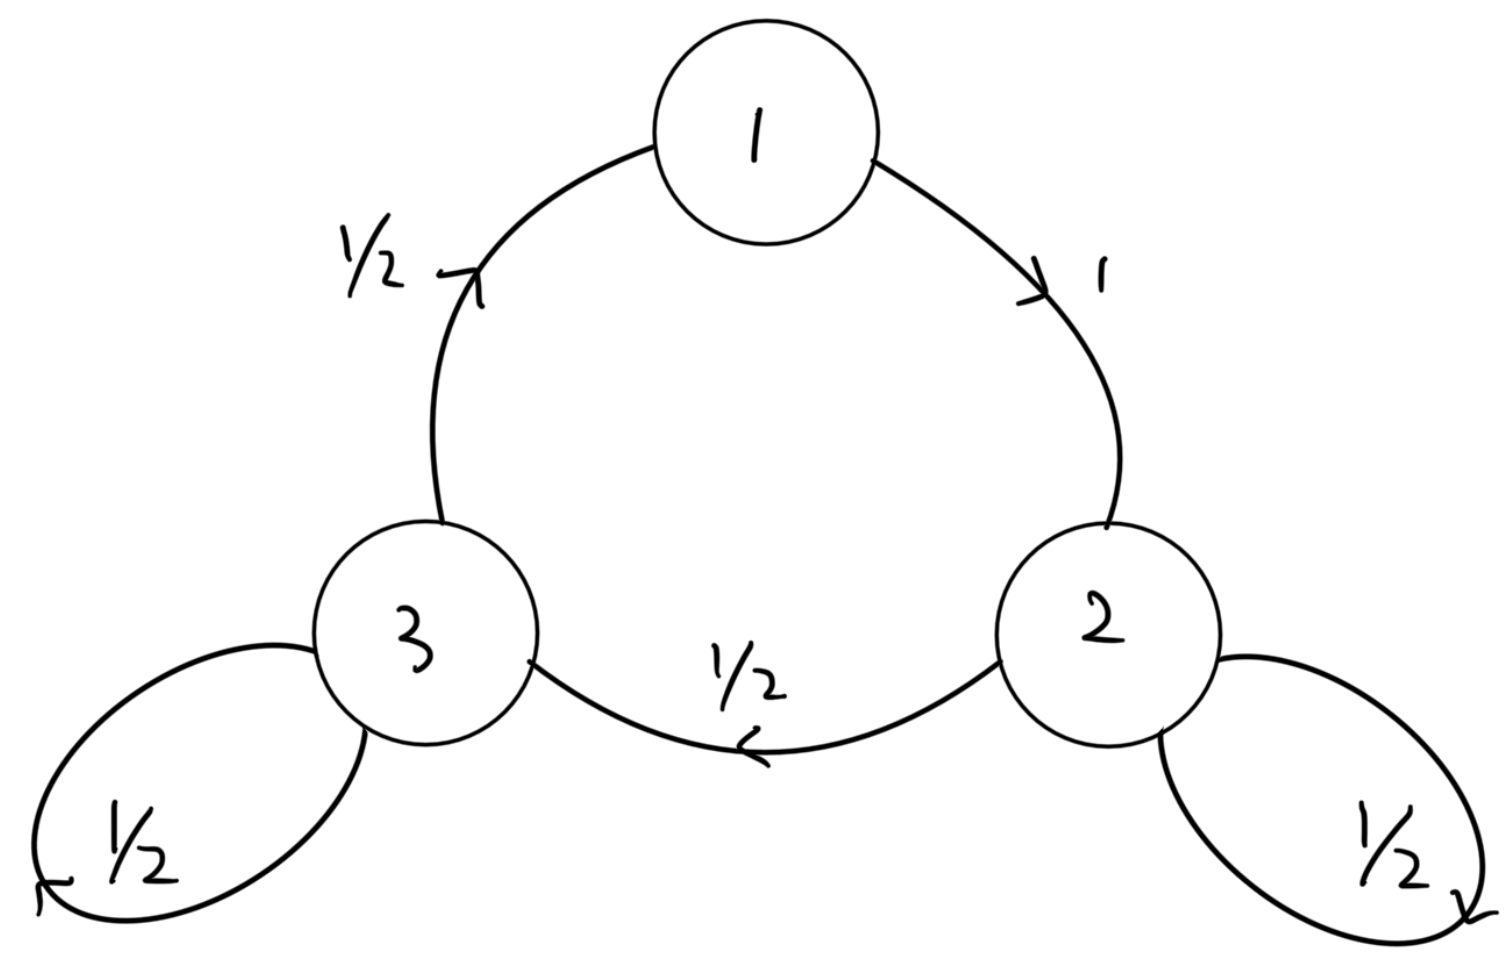
\includegraphics[width=0.7\textwidth]{fig/markov-chain-eigenvalues-matrix.png}
    \caption{Markov Chain in \autoref{ex:markov-chain-eigenvalues}}
    \label{fig:markov-chain-eigenvalues}
\end{figure}